\documentclass[12pt]{article}

\usepackage[spanish]{babel}
\usepackage[utf8]{inputenc}
\usepackage{graphicx}
\usepackage{geometry}
\usepackage{xcolor}
\usepackage{fancyhdr}
\usepackage{lastpage}
\usepackage{pdfpages}
\usepackage{listings}

\geometry{top=25mm,left=15mm,right=15mm,a4paper}

\pagestyle{fancy}
\fancyhf{}
\lhead{Seminario de Ciencias de la Computación A}
\cfoot{Página \thepage\ de \pageref{LastPage}}

\graphicspath{./}

\begin{document}
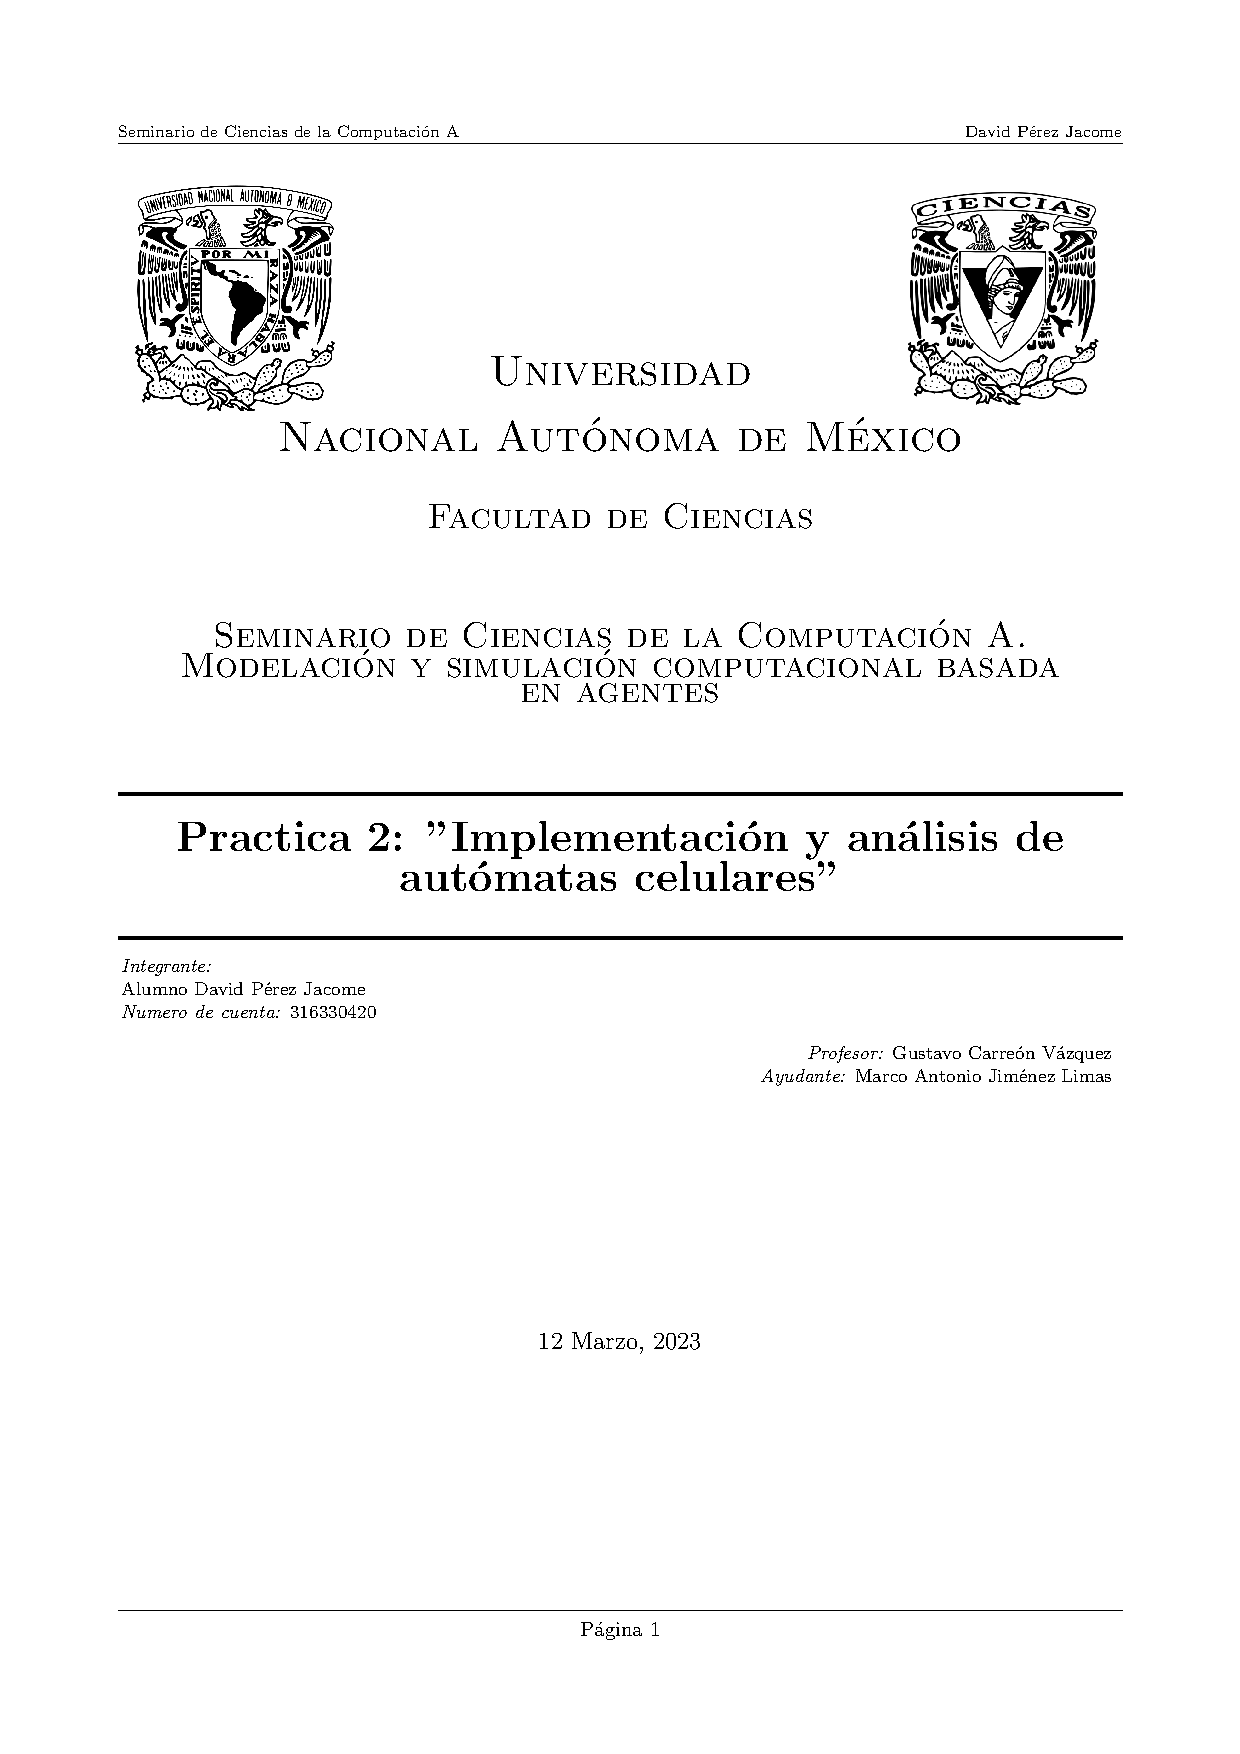
\includepdf{Portada.pdf}
{\color{red} \section*{Practica 3: Modelación de una dinámica de epidemias
con MBA.}}
\vspace{2em}

{\color{blue} \subsection*{Parte 1. Modelo basado en agentes SIR con distanciamiento social.}}
\vspace{1em}

Cada vez son más utilizados los modelos y simulaciones computacionales para recrear escenarios de los fenómenos y tomar mejores
decisiones. La actual pandemia que estamos viviendo requiere de su estudio y análisis desde distintos enfoques. Con la modelación
basada en agentes se puede entender la estrategia de distanciamiento social, su efectividad e impacto en la disminución de casos a lo
largo del tiempo. En el árticulo de Harry Stevens se propone un modelo para explicar los beneficios del distanciamiento social en una dinámica de contagio.\\

\textbf{Implementación del modelo en NetLogo}\\

El sistema se compone de una reticula de $n$ x $n$ donde $n=100$. Se colocan $k$ agentes (personas) distribuidos aleatoriamente sobre el sistema.\\

Estas personas pueden estar en uno de tres posibles estados: \textbf{sano, enfermo o recuperado}. Asigne un color para visualizar, por ejemplo, \textbf{sano=azul}, \textbf{enfermo=rojo} y \textbf{recuperado=verde}.
Las personas son caminadores aleatorios con un rango de visión determinado.\\

\textbf{Reglas:}\\

\begin{enumerate}
    \item \textbf{Contagio:} Si una persona sana tiene una persona enferma en su vecindad de Moore entonces se contagia con cierta probabilidad y cambia su estado a enfermo. Una persona
    enferma no puede contagiar nuevamente a una persona recuperada.
    \item \textbf{Recuperación:} Una persona enferma se recupera después de $k$ tiempos y cambia su estado a recuperado.
    \item \textbf{Movimiento:} Las personas son caminantes aleatorios con un rango de visión determinado (por ejemplo $-60$ y $60$ grados).
    \item \textbf{Distanciamiento social:} El distanciamiento social es una estrategia para mitigar los efectos de contagio en una pandemia. Las personas se exponen lo menos posible en lugares concurridos. En el modelo, las personas que
    apliquen distanciamiento social no se moverán como en el artículo de Harry Stevens.
\end{enumerate}

\textbf{Parámetros globales:}\\

Los parametros globales determinan el comportamiento del sistema y tiene un rango para establecer los valores:\\

\begin{enumerate}
    \item Densidad de la población \textbf{(POB)} de $10$ a $100\%$ en función del número de patches en el mundo.
    \item Apertura de visión del agente \textbf{(WIG)} de $10$° a $360$°.
    \item Probabilidad de contagio \textbf{(PC)}, se establece en el intervalo $0$ a $1$. Los casos extremos son: si es $0$ la persona infectada no puede transmitir la enfermedad; si es $1$ la persona infectada
    transmite la infección inmediatamente.
    \item Tiempo de la enfermedad \textbf{(TE)} de $10$ a $100$ tiempos o tiks.
    \item Distanciamiento social\textbf{(DS)} de $10$ a $100\%$ de la población, es el porcentaje de la población que hace distanciamiento social.
\end{enumerate}

{\color{blue} \subsubsection*{Experientos.}}
\vspace{1em}

\begin{enumerate}
    \item 
\end{enumerate}





\end{document}